%%%%%%%%%%%%%%%%%%%%%%% file MESON2018_YourName_paper.tex %%%%%%%%
%
% This is a template file for Web of Conferences Journal
%
% Copy it to a new file with a new name and use it as the basis
% for your article
%
%%%%%%%%%%%%%%%%%%%%%%%%%% EDP Science %%%%%%%%%%%%%%%%%%%%%%%%%%%%
%
%%%\documentclass[option]{webofc}
%%% "twocolumn" for typesetting an article in two columns format (default one column)
%
\documentclass[epj]{webofc}
\usepackage[varg]{txfonts}   % Web of Conferences font
\usepackage{graphicx}
\usepackage{subcaption}
%
% Put here some packages required or/and some personnal commands
%
\woctitle{MESON2018 - the 15$^\textrm{th}$ International Workshop on Meson Physics}
%
\begin{document}
%
\selectlanguage{english}
\title{Recent results of quarkonium and heavy flavour at ATLAS}

% insert email only for speaker/presenter
\author{Weimin~Song\inst{1}\fnsep\thanks{\email{wesong@cern.ch}}
% comment out the next line if not needed
       \\for the ATLAS Collaboration
}

\institute{Particle Physics Department, Rutherford Appleton Laboratory, Didcot, UK
          }

\abstract{%Do not break line here!
Heavy quark spectroscopy and exotic states are studied with the ATLAS detector, mainly
thorough final states containing muon pairs from $J/\psi$ decays from both proton-proton,
proton-lead and lead-lead collisions. This proceedings will summarise recent results from ATLAS,
including production of quarkonium and heavy flavour, searches for exotic states and
measurements of decay properties in open beauty production.
}
%
\maketitle
%
\section{Introduction}
\label{intro}

Hardons have been used to test the particle physics Standard Model (SM) for a long time.
%In the current days, they are still crutial for particle physics, for examle by measuring the decay rate
%of $B_s \to \mu^{+}\mu^{-}$, the SM could be checked in a very high precision.
The heavy flavour hadrons are massly produced in the proton proton collisions at Large Hadron Collider.
With ATLAS detector, the production and decay of the heavy flavour hadrons could be studied. 
When comparing with the other detectors which are optimised for hadron physics study, such as Belle (II), BESIII, and
LHCb, the advantage of ATLAS is that the number of recorded hardons is larger, while the disadvantage is the particle identification 
system is not designed for the seperation between different hadrons. 
Normally, the $J/\psi \to \mu^{+} \mu^{-}$ is required in the final state, in order to reduce the background, which is much more
higher in the hadron collider when comparing with electron-positron collider.\\ 

In this proceddings, four recent publications from ATLAS are discussed, they are:
\begin{itemize}
  \item Search for a Structure in the $B^0_s \pi^\pm$ Invariant Mass Spectrum with the ATLAS Experiment~\cite{x5568}
  \item Measurement of $b$-hadron pair production with the ATLAS detector in proton-proton collisions at $\sqrt{s}=8$ TeV~\cite{bpair}
  \item Measurement of quarkonium production in proton–lead and proton–proton collisions at $5.02~\mathrm {TeV}$ with the ATLAS detector~\cite{quark_pro}
  \item Angular analysis of $B^0_d \rightarrow K^{*}\mu^+\mu^-$ decays in $pp$ collisions at $\sqrt{s}= 8$ TeV with the ATLAS detector~\cite{kmumu}
\end{itemize}

\section{Is X(5568) observed in the ATLAS dataset?}
\label{5568}

In 2016, with 10.4~$fb^{-1}$ proton anti-proton collision data at center of mass energy of 1.96 TeV, the D0 collaboration made a claim about
the discovery of X(5568) in the $B^0_s \pi^\pm$ final states~\cite{D0:2016mwd}. The structure was interpreted as a tetraquark with four 
different quark flavors: b, s, u and d. However, with similar method and same final state topology, neither CMS~\cite{Sirunyan:2017ofq}, LHCb~\cite{Aaij:2016iev} 
at LHC nor CDF~\cite{Aaltonen:2017voc} at Tevetran find any hint of X(5568).   

AT ALTAS, the analysis is based on a data sample recorded with the ATLAS detector at the LHC corresponding to 4.9 
$fb^{-1}$ of pp collisions at 7 TeV and 19.5 $fb^{-1}$ at 8 TeV.
No significant signal was found, as shown by Fig.~\ref{fig:5568}. Upper limits on the number of signal events, with properties corresponding to 
those reported by D0, and on the X production rate relative to $B_{s}^{0}$ mesons, $\rho~X$, were determined at 95\% confidence level. 
The results are N(X)<382 and $\rho~X$<0.016 for $B_{s}^{0}$ mesons with transverse momenta above 10 GeV, and N(X)<356 and $\rho~X$<0.017 for 
transverse momenta above 15 GeV. 

\begin{figure}
    \centering
    \begin{subfigure}[h]{0.45\textwidth}
        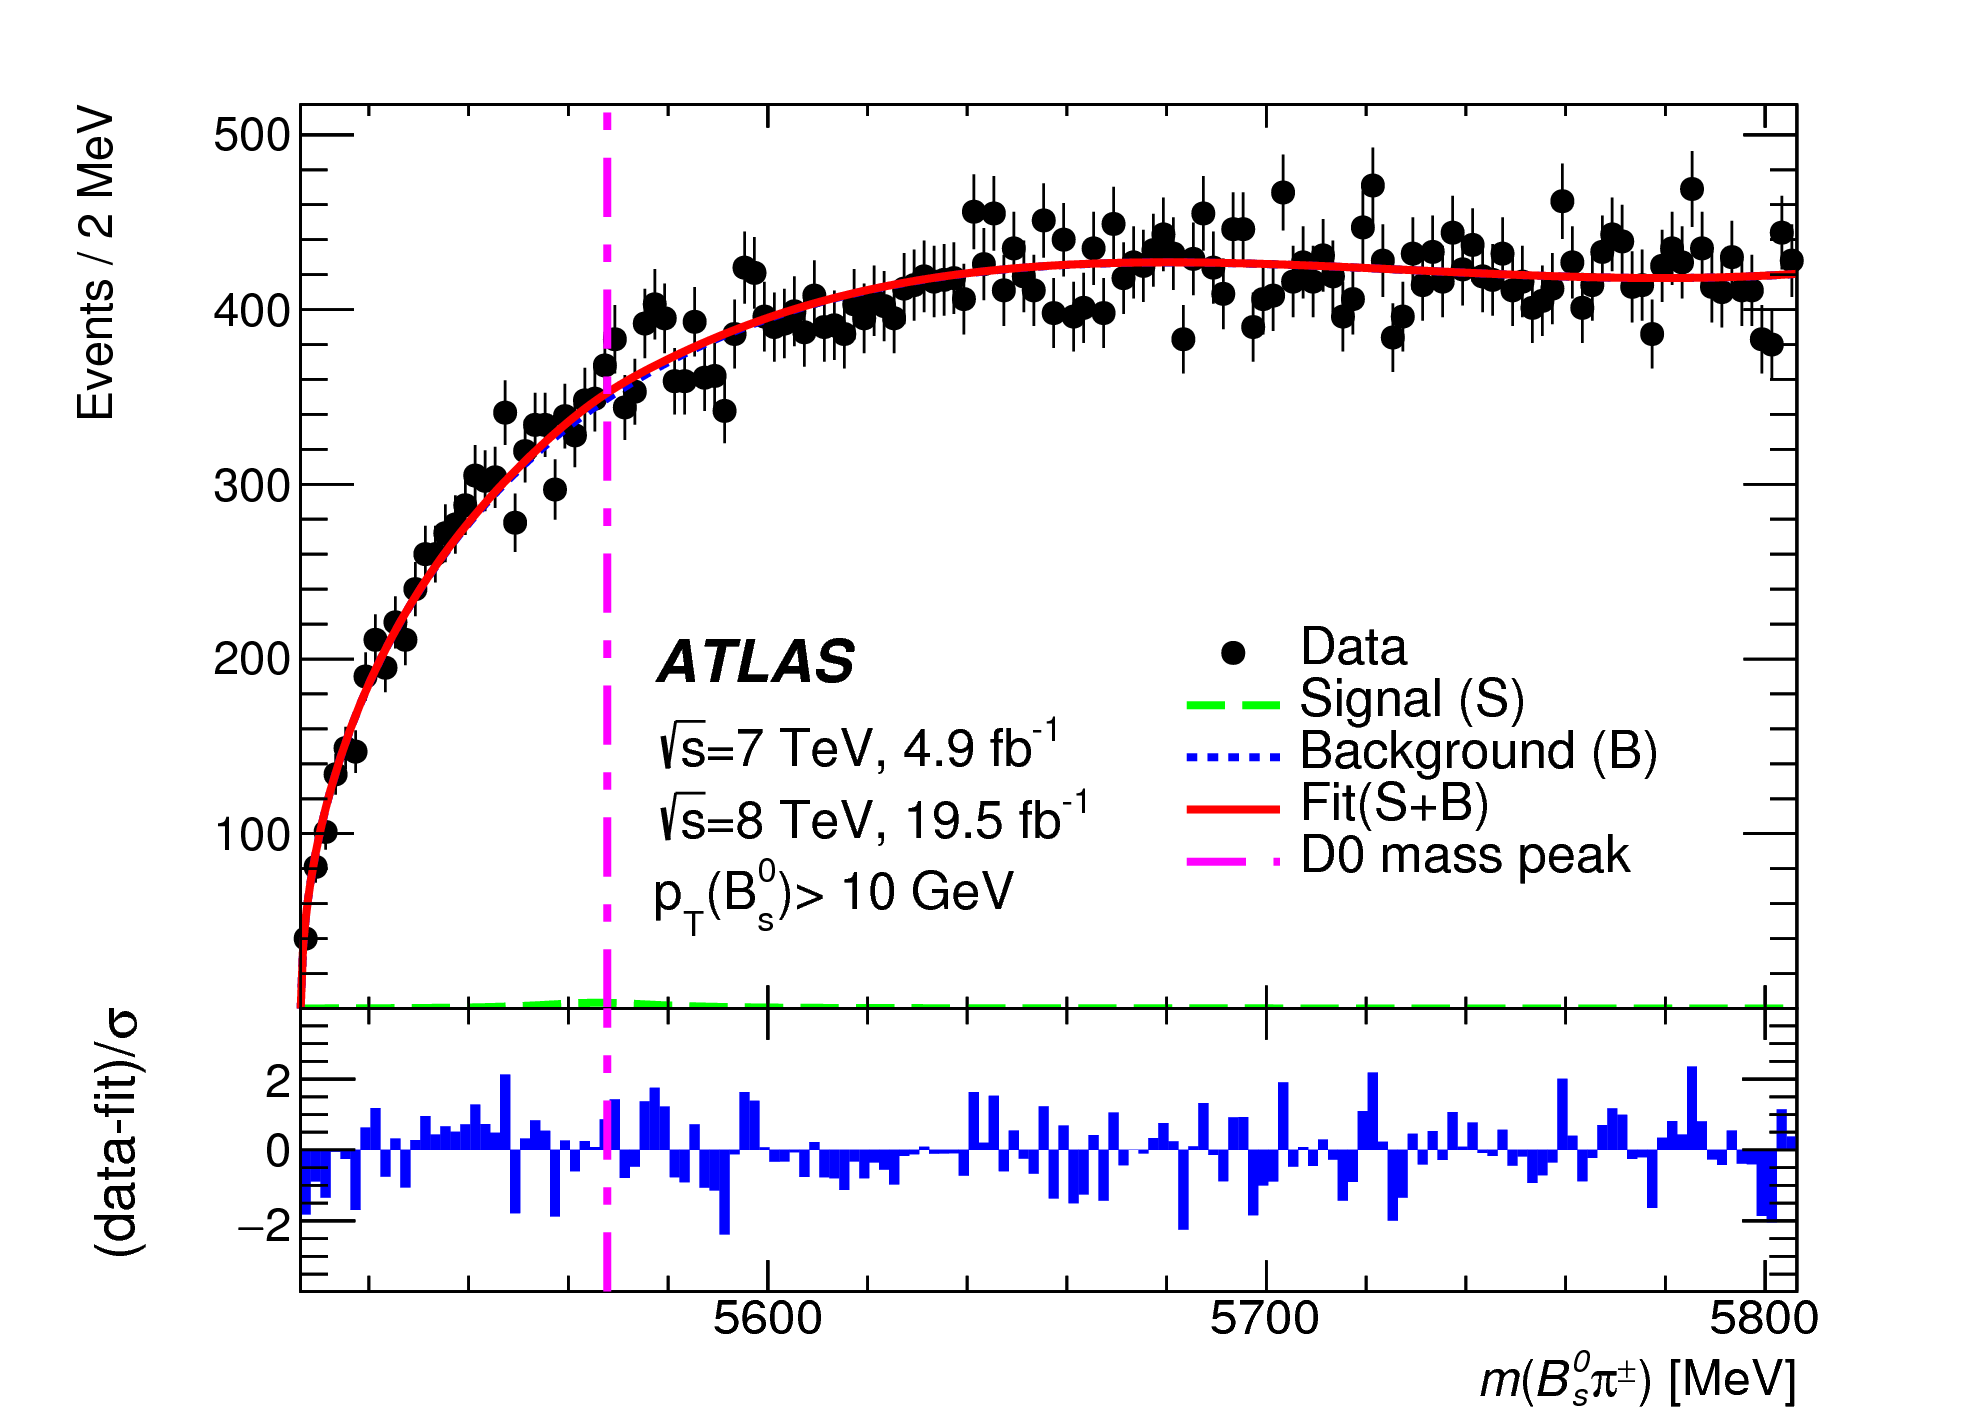
\includegraphics[width=\textwidth]{plots/5568/fig_02a.png}
    \end{subfigure}
    \begin{subfigure}[h]{0.45\textwidth}
        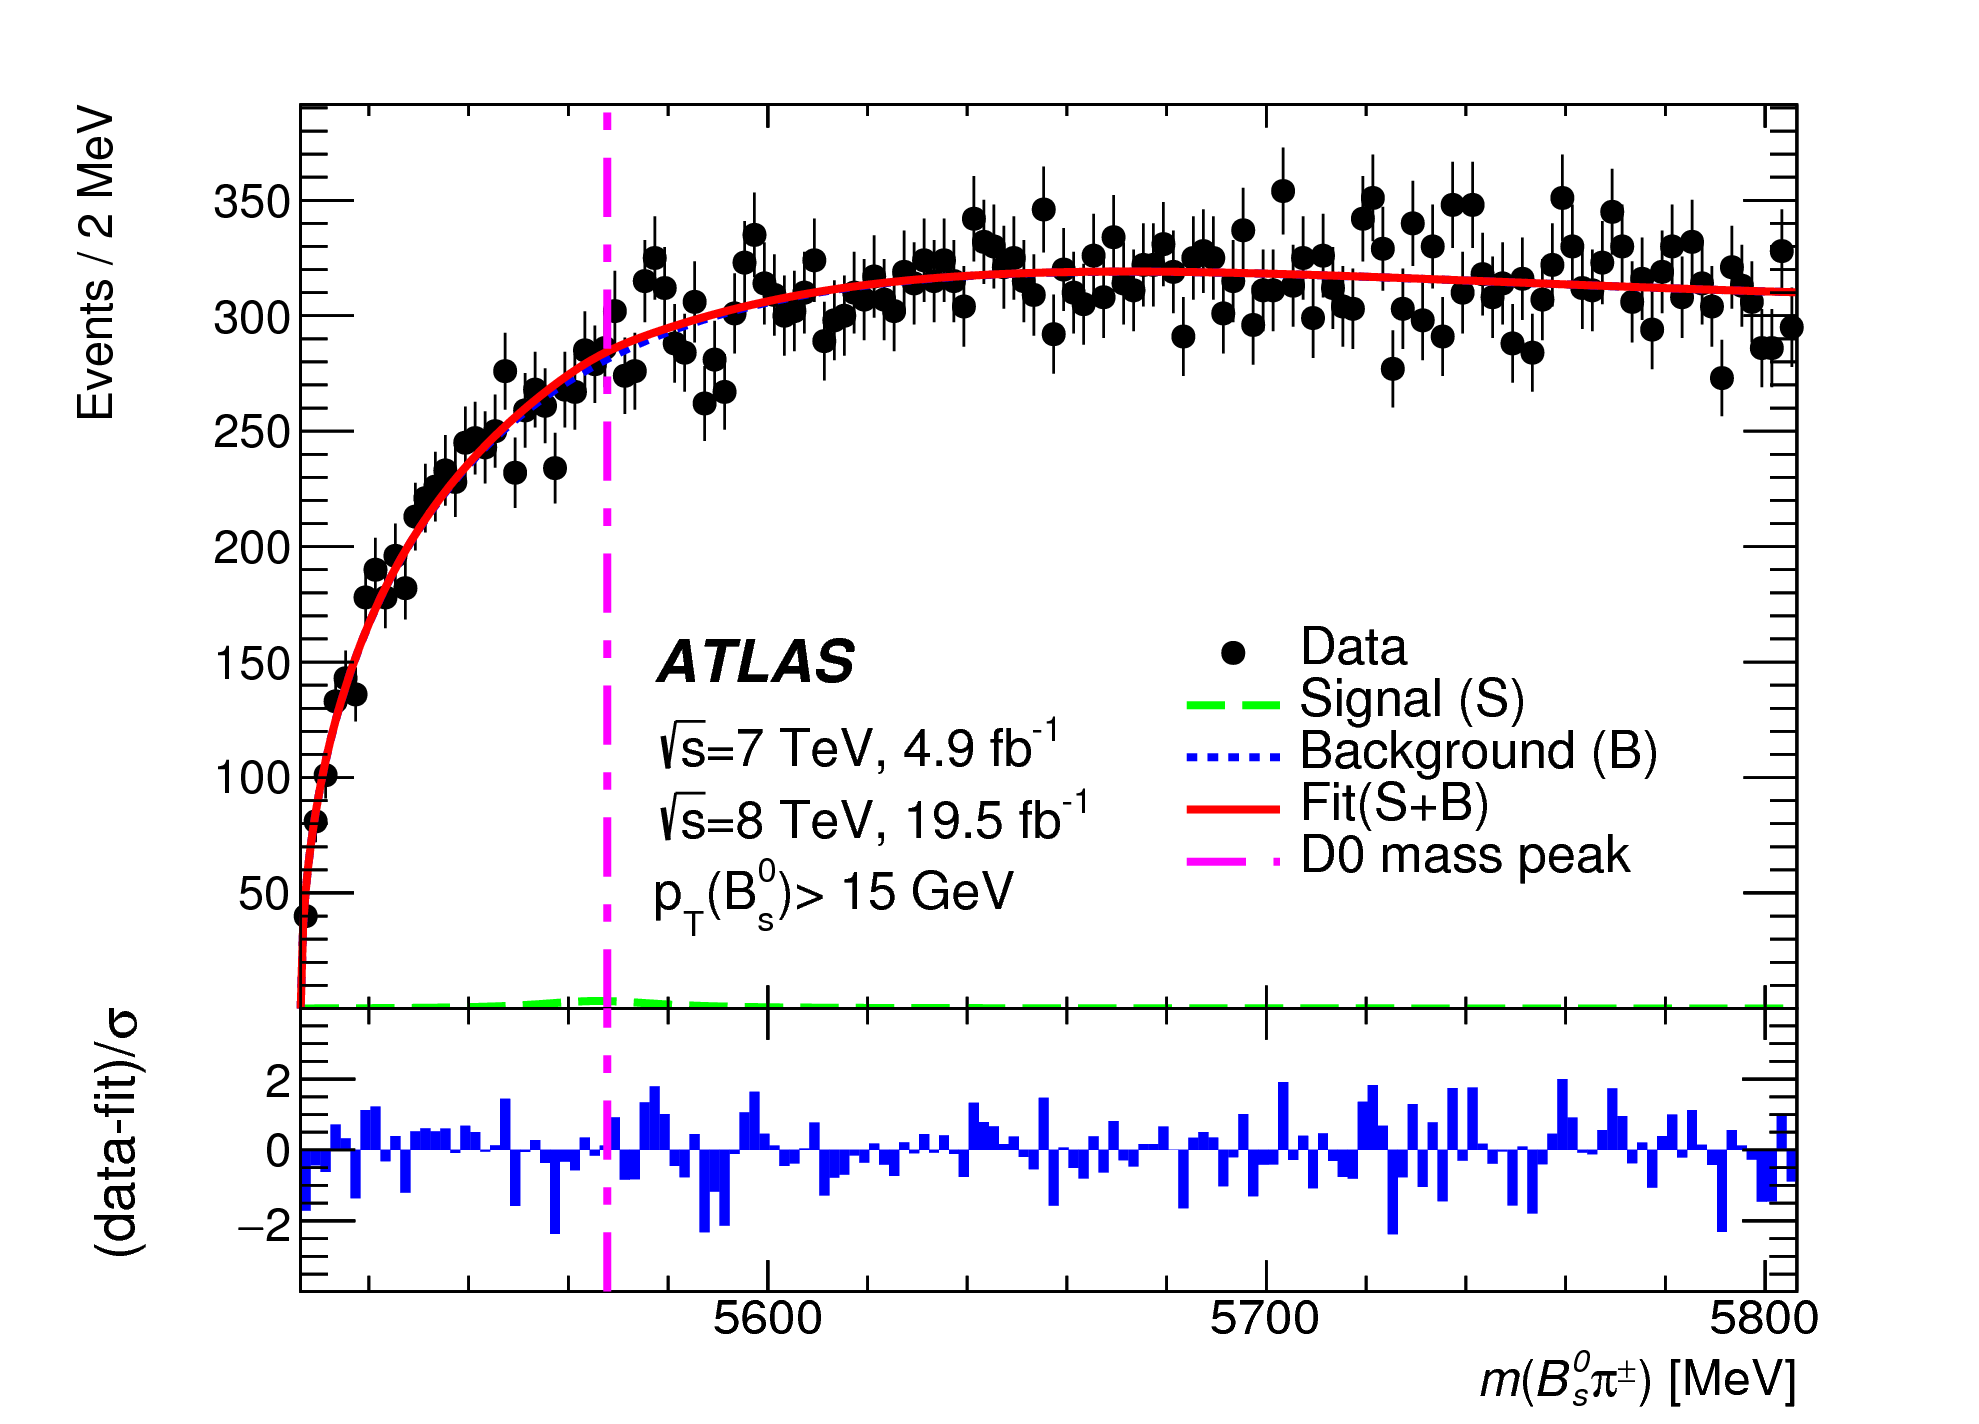
\includegraphics[width=\textwidth]{plots/5568/fig_02b.png}
    \end{subfigure}
    \caption{$B_{s}^{0}\pi^{\pm}$ mass distribution for candidates with $p_T$($B_{s}^{0}$)>10 GeV (left) and $p_T$($B_{s}^{0}$)>15 GeV (right). 
     The bottom panels show the difference between each data point and the fit divided by the statistical uncertainty of that point.}
    \label{fig:5568}
\end{figure}

The reason that the particle is observed by one experiment but not the other experiment could be physics also, rather than the mistakes
made by experiments, as discussed by~\cite{Yang:2016sws}\cite{Ke:2018stp}. More study is needed about the X(5568) on bothe experimental and theoritical side. 


\section{$b$-hadron pair production}

The production of heavy flavour quark in proton–proton collisions provides a fruitful testing ground for the predictions of quantum chromodynamics (QCD).
There are a few methods that could be used to identify the heavy flavour quark, which will become a jet, in experiment. 
One popular method is based on the presence of a decay vertex orcharged-particle tracks displaced from the primary interaction vertex 
due to the lifetime of the b-hadron, for example in~\cite{Aaboud:2016jed}. The disadvantage of this method is that when the angle
between two heavy flavour quark is small, the performance of the tagging algorithm is poor due to the bad worse vetex fitting resolution. 

ATLAS collaboration performed a new measurement of the production of two b-hadrons by tagging one b-hadron with $J\psi (\to \mu \mu)$+X and the other with $\mu$ + Y, 
resulting in three muons in the final state. This means that the signature of the signal is: non-prompt $J\psi$ decaying to two muons, and an third muon from the same
interaction point.

 

\section{Summary}
\label{sum}

\begin{acknowledgement}

\end{acknowledgement}
%
% BibTeX or Biber users please use (the style is already called in the class, ensure that the "woc.bst" style is in your local directory)
% \bibliography{name or your bibliography database}
%
% Non-BibTeX users please use
%
\begin{thebibliography}{00}
%
% and use \bibitem to create references.
%
\bibitem{x5568}
  M.~Aaboud {\it et al.} [ATLAS Collaboration],
  %``Search for a Structure in the $B^0_s \pi^\pm$ Invariant Mass Spectrum with the ATLAS Experiment,''
  Phys.\ Rev.\ Lett.\  {\bf 120}, no. 20, 202007 (2018)
\bibitem{bpair}
  M.~Aaboud {\it et al.} [ATLAS Collaboration],
  %``Measurement of $b$-hadron pair production with the ATLAS detector in proton-proton collisions at $\sqrt{s}=8$ TeV,''
  JHEP {\bf 1711}, 062 (2017)
\bibitem{quark_pro}
  M.~Aaboud {\it et al.} [ATLAS Collaboration],
  %``Measurement of quarkonium production in proton–lead and proton–proton collisions at $5.02~\mathrm {TeV}$ with the ATLAS detector,''
  Eur.\ Phys.\ J.\ C {\bf 78}, no. 3, 171 (2018)
\bibitem{kmumu}
  M.~Aaboud {\it et al.} [ATLAS Collaboration],
  %``Angular analysis of $B^0_d \rightarrow K^{*}\mu^+\mu^-$ decays in $pp$ collisions at $\sqrt{s}= 8$ TeV with the ATLAS detector,''
  arXiv:1805.04000 [hep-ex].
%\cite{D0:2016mwd}
\bibitem{D0:2016mwd} 
  V.~M.~Abazov {\it et al.} [D0 Collaboration],
  %``Evidence for a $B_s^0 \pi^\pm$ state,''
  Phys.\ Rev.\ Lett.\  {\bf 117}, no. 2, 022003 (2016)
%\cite{Sirunyan:2017ofq}
\bibitem{Sirunyan:2017ofq} 
  A.~M.~Sirunyan {\it et al.} [CMS Collaboration],
  %``Search for the X(5568) state decaying into $\mathrm{B}^{0}_{\mathrm{s}}\pi^{\pm}$ in proton-proton collisions at $\sqrt{s} = $ 8 TeV,''
  Phys.\ Rev.\ Lett.\  {\bf 120}, no. 20, 202005 (2018)
%\cite{Aaij:2016iev}
\bibitem{Aaij:2016iev} 
  R.~Aaij {\it et al.} [LHCb Collaboration],
  %``Search for Structure in the $B_s^0\pi^\pm$ Invariant Mass Spectrum,''
  Phys.\ Rev.\ Lett.\  {\bf 117}, no. 15, 152003 (2016)\\
  Addendum: [Phys.\ Rev.\ Lett.\  {\bf 118}, no. 10, 109904 (2017)]
%\cite{Aaltonen:2017voc}
\bibitem{Aaltonen:2017voc} 
  T.~Aaltonen {\it et al.} [CDF Collaboration],
  %``A search for the exotic meson $X(5568)$ with the Collider Detector at Fermilab,''
  Phys.\ Rev.\ Lett.\  {\bf 120}, no. 20, 202006 (2018)
%\cite{Yang:2016sws}
\bibitem{Yang:2016sws} 
  Z.~Yang, Q.~Wang and U.~G.~Meißner,
  %``Where does the X(5568) structure come from?,''
  Phys.\ Lett.\ B {\bf 767}, 470 (2017)
%\cite{Ke:2018stp}
\bibitem{Ke:2018stp} 
  H.~W.~Ke and X.~Q.~Li,
  %``How can $X^{\pm}(5568)$ escape detection?,''
  arXiv:1802.08823 [hep-ph].
%\cite{Aaboud:2016jed}
\bibitem{Aaboud:2016jed} 
  M.~Aaboud {\it et al.} [ATLAS Collaboration],
  %``Measurement of the $b\overline{b}$ dijet cross section in pp collisions at $\sqrt{s} = 7$  TeV with the ATLAS detector,''
  Eur.\ Phys.\ J.\ C {\bf 76}, no. 12, 670 (2016)
\end{thebibliography}

\end{document}

% end of file template.tex

<div id='footer'><table width='100%'><tr><td class='right'><a href='http://fusioninventory.org/'><span class='copyright'>FusionInventory 9.1+1.0 | copyleft <img src='/glpi/plugins/fusioninventory/pics/copyleft.png'/>  2010-2016 by FusionInventory Team</span></a></td></tr></table></div>
